\documentclass[10pt]{beamer}
\usetheme{metropolis}           % Use metropolis theme

\usepackage{appendixnumberbeamer}

\usepackage{pgfpages}
%\setbeamertemplate{note page}[plain]
%\setbeameroption{show notes on second screen=right}
\makeatletter 
% the following fixes bug which causes normal text to be white instead of
% template default when notes are enabled
% (see https://tex.stackexchange.com/questions/232168/normal-text-is-invisible-when-using-beamer-with-notes-and-xelatex)
\def\beamer@framenotesbegin{% at beginning of slide
     \usebeamercolor[fg]{normal text}
      \gdef\beamer@noteitems{}% 
      \gdef\beamer@notes{}% 
}
\makeatother

\usepackage[scale=3]{ccicons}   % creative commons icons

\title{CSCI 160 --- Introduction to Problem-solving \& Programming}
\date{}
\author{Jeremy Iverson}
\institute{College of Saint Benedict \& Saint John's University}
\begin{document}
  \maketitle

  \begin{frame}{logistics}
    \begin{itemize}
      \item instructor(s)
        \begin{itemize}
          \item Jeremy Iverson (\href{mailto:jiverson002@csbsju.edu}{\nolinkurl{jiverson002@csbsju.edu}})
          \item PENGL 213, (320) 363-5542
          \item office hours: \begin{tabular}[t]{rrrcr}
                                T & 10:00 & - & 11:00 \\
                                W & 14:00 & - & 15:00
                              \end{tabular}
        \end{itemize}
      \item textbook
        \begin{itemize}
          \item \emph{Java Early Objects}, Lysecky and Lizarraga et al., zyBook
        \end{itemize}
      \item website
        \begin{itemize}
          \item \url{https://csbsju.instructure.com/courses/13506}
        \end{itemize}
      \item labs
        \begin{itemize}
          \item PENGL 218, TR \begin{tabular}[t]{rrcr}
                                01A & 09:30 & - & 10:25 \\
                                02A & 13:00 & - & 13:55
                              \end{tabular}
        \end{itemize}
    \end{itemize}

    \note{I prefer to be called Jeremy\\}
    \note{Encourage questions right away\\}
    \note{Emphasize the importance of the Canvas site for finding information
      about the class}
  \end{frame}

  \begin{frame}{course objectives}
    \begin{itemize}
      \item write well-designed Java programs for small-scale problems
      \item identify appropriate object classes for solving a given problem
      \item write good documentation for programs
    \end{itemize}

    \note{Will not be asked to write full-scale applications
      \begin{itemize}
        \item Emphasizes programming fundamentals, special attention to
          object-oriented software design (ptyon and visual basic are both
          examples)
        \item Problem-solving
      \end{itemize}
    }
  \end{frame}

  \begin{frame}{course content}
    \begin{itemize}
      \item introduction to Java
      \item using methods
      \item using objects
      \item decisions
      \item iterations
      \item arrays
      \item designing and implementing classes
      \item inheritance
      \item interfaces and polymorphism
      \item file i/o
      \item exceptions
      \item recursion
      \item searching
      \item sorting
      \item collections
      \item advanced topics
    \end{itemize}

    \note{Ask students to point out some of the topics which are covered in
      130/150\\}
    \note{Point out that each of these bullets corresponds to one of the
      ``modules'' on Canvas}
  \end{frame}

  \begin{frame}{technologies}
    \begin{itemize}
      \item Java - language
      \item Dr. Java - integrated development environment
      \item Linux - operating system
      \item Github - source code management platform
      \item Canvas - learning management system
      \item Outlook - calendar management application
      \item maybe others\dots
    \end{itemize}

    \note{\begin{itemize}
      \item I will be sure to remind for the first couple labs, after that
      \item Your responsibility to go on N drive to course folder to see if
        there is a prelab
      \item I will try to remind, but it is student’s responsibility
      \item Amounts to two (roughly 30 min) assignments per week
      \item Labs are due Tuesday following the lab session that they are
        assigned
    \end{itemize}}
  \end{frame}

  \begin{frame}{labs}
    \begin{itemize}
      \item attendance
      \item prelabs
    \end{itemize}

    \note{\begin{itemize}
      \item I will be sure to remind for the first couple labs, after that
      \item Your responsibility to go on N drive to course folder to see if
        there is a prelab
      \item I will try to remind, but it is student’s responsibility
      \item Amounts to two (roughly 30 min) assignments per week
      \item Labs are due Tuesday following the lab session that they are
        assigned
    \end{itemize}}
  \end{frame}

  \begin{frame}{assignments}
    \begin{itemize}
      \item do your own work
      \item use each other as resources only
    \end{itemize}

    \note{Should be student's own work, may work together but must individual
      solutions\\}
    \note{Want to encourage using each other as resources, but do not want some
      students to rely on other students for answers}
  \end{frame}

  \begin{frame}{quizzes and exams}
    \begin{itemize}
      \item three (3) lab quizzes (open book / note)
      \item two (2) in-class exams (closed book / note)
      \item one (1) in-class final exam (closed book / open note) [cumulative]
    \end{itemize}

    \note{Make-up exams are possible under certain circumstances, but no make-up
      quizzes}
  \end{frame}

  \begin{frame}{office hours}
    \begin{itemize}
      \item stop by anytime
      \item \href{http://exchange.csbsju.edu/owa/calendar/JIVERSON002@CSBSJU.EDU/Calendar/calendar.html}{my calendar}
    \end{itemize}

    \note{Mention outlook calendar \& my home page\\}
    \note{For those unfamiliar with Outlook meetings, then they should schedule
      another way and we will go over this in meeting\\}
    \note{Mention not generally availability in the afternoons}
  \end{frame}

  \begin{frame}{expectations}
    \begin{itemize}
      \item prepare for class (do the reading!)
      \item participate in class
      \item be respectful
    \end{itemize}

    \note{\begin{itemize}
      \item Don’t just read, by try your best to make sense of the material
      \item Emphasize that students are not just recipients of my knowledge ---
        they can shape the direction of the course
      \item Encourage students to stop and think before replying.
      \item Don’t be discouraged if comprehension is not apparent right away,
        but don’t be complacent
      \item \textbf{Seek help (TAs and me)}
      \item Students can expect the same things from me.
    \end{itemize}}
  \end{frame}

  \begin{frame}[standout]
    \usebeamercolor[white]{normal text} % override bug fix in preamble
    questions?
  \end{frame}

  \appendix

  \begin{frame}{notecards}
    \begin{itemize}
      \item upcoming assignment will be to schedule a 10 minute meeting with me
        in my office to handle introductions
    \end{itemize}
  \end{frame}

  \begin{frame}{Java program}
    \begin{itemize}
      \item open \href{https://gist.github.com/jiverson002/19b476e9142ccff16b01f0692fa58666\#file-lecture1-java}{Lecture1.java}
      \item follow the instructions
    \end{itemize}
  \end{frame}

  \begin{frame}
    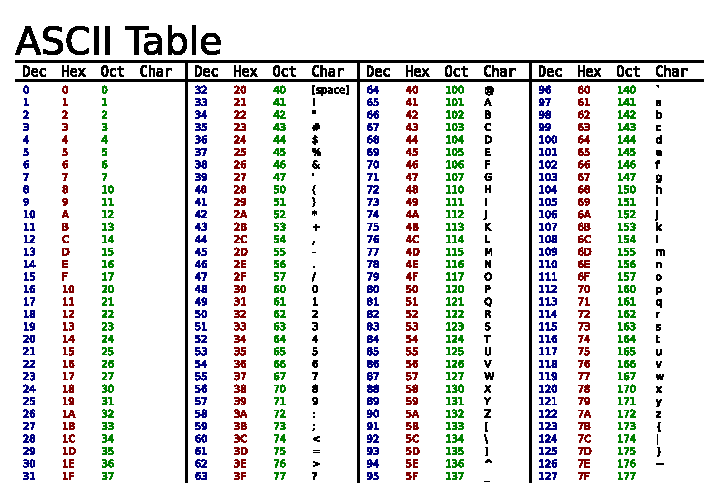
\includegraphics[width=\textwidth]{Ascii-proper-color}
  \end{frame}

  \begin{frame}
    \begin{center}\ccbysa\end{center}

    except where otherwise noted, this worked is licensed under
    \href{http://creativecommons.org/licenses/by-sa/4.0/}{creative commons
    attribution-sharealike 4.0 international license}
  \end{frame}
\end{document}
